\documentclass[12pt,a4paper]{article}
\usepackage{polski}
\usepackage[polish]{babel}
\usepackage{bbm}
\usepackage{bm}
\usepackage[T1]{fontenc}
\usepackage[utf8]{inputenc}
\usepackage[top=2cm, bottom=2cm, left=3cm, right=3cm]{geometry}
\usepackage{url}
\usepackage{graphics}
%\usepackage{graphicx}
\usepackage[pdftex]{graphicx}
\usepackage{float}
\usepackage{amsmath,amsthm}
\usepackage{enumitem}
\usepackage{epstopdf}
%\usepackage{indentfirst}
\usepackage[labelsep=period]{caption}
\setlist{nolistsep}


\AtBeginDocument{% Fragment zmieniający nazwy 'Rysunek' na 'Wykres' i 'Tablica' na 'Tabela'
        \renewcommand{\tablename}{Tabela}
        \renewcommand{\figurename}{Wykres}
}

\makeatletter
\newcommand{\linia}{\rule{\linewidth}{0.4mm}}


\floatstyle{plain}
\newfloat{image}{h!}{lop}
\floatname{image}{Rysunek}



\let \savenumberline \numberline
\def \numberline#1{\savenumberline{#1.}}


\renewcommand*{\@seccntformat}[1]{%
	  \csname the#1\endcsname
		    .\quad
}


\renewcommand{\maketitle}{\begin{titlepage}
		\vspace*{1cm}
    \begin{center}\small
    	Uniwersytet Wrocławski\\
    	Wydział Matematyki i Informatyki\\
    \end{center}
    \vspace{3cm}
    \noindent
    \linia
    \begin{center}
    	\LARGE{\textsc{\@title}}
         \end{center}
     \linia
    \begin{center}
    	\Large{Opis interfejsów}
         \end{center}
    \vspace{0.5cm}

    \begin{flushright}

    \begin{minipage}{5.5cm}

    	\small Autorzy:

    \normalsize {\@author} \par
    

    \end{minipage}
    \vspace{5cm}

     

     \end{flushright}

    \vspace*{\stretch{6}}

    \begin{center}

    \@date\\

    \end{center}

  \end{titlepage}%

}


\makeatother

\author{Jakub Stępniewicz (\textbf{233217})\\Rafał Maćkowski (\textbf{233170})\\Grupa {\bf I}}

\title{Symulator tramwaju\\ \small{Też możesz być motorniczym}}


\begin{document}
\maketitle
\tableofcontents
\vspace{5cm}
%	\begin{thebibliography}{9}
%	\bibitem{US} tz, W. Hill {\it Us}, Warszawa 2009.
%	\bibitem{MPK} \url{http://www.mpk.wroc.pl/}
%	\bibitem{SK} \url{http://www.skoda.cz/en/products/tramcars/tramcar-19-t/}
%	\bibitem{UE} \url{http://www.unrealengine.com/}
%	\bibitem{GO} \url{http://www.google.pl/#sclient=psy-ab&hl=pl&source=hp&q=%22symulator+tramwaju+skoda+16t%22&pbx=1&oq=%22symulator+tramwaju+skoda+16t}
%	\end{thebibliography}
\newpage
% 		Ok, najtrudniejsze za nami.		%
% 

\section{Wstęp}
Dokument zawiera opis interfejsów symulatora. Są to:
\begin{itemize}
\item interfejs motorniczego,
\item interfejs instruktora,
\item sieciowy interfejs administracyjny.
\end{itemize}
\section{Opis interfejsów}
W następnych rozdziałach zostaną opisane podstawowe cechy poszczególnych interfejsów.
\subsection{Interfejs motorniczego}
Interfejs motorniczego został przedstawiony na rysunku \ref{cock}. Opis poszczególnych elementów znajduje się w tabeli \ref{opis} (strona \pageref{opis}).
\begin{image}[p!]
	\begin{center}
		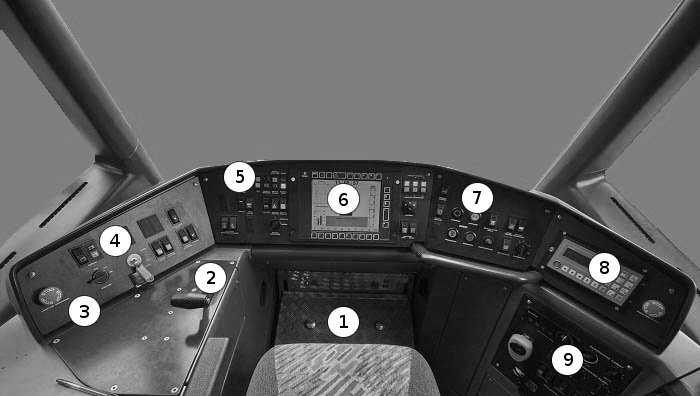
\includegraphics[bb=0 0 700 396]{img/cockNUM.jpg}
		\caption{Kokpit tramwaju {\it Škoda 19T}}
			\label{cock}
	\end{center}
\end{image}

\begin{table}[p!]
\caption{Opis elementów kokpitu}
	\begin{center}
\begin{tabular}{l|l}
\texttt{Numer} & \texttt{Opis} \\ \hline
1.&Czuwak aktywny\\
2.&Przepustnica\\
3.&Przełącznik hamulca awaryjnego\\
4.&Stacyjka\\
5.&Sterowanie oświetlenia i ogrzewania\\
6.&Wyświetlacz wielofunkcyjny\\
7.&Sterowanie drzwiami\\
8.&GPS i ustawienia trasy\\
9.&Radiotelefon\\
\end{tabular}
\label{opis}
\end{center}
\end{table}
\subsection{Interfejs instruktora}
Interfejs instruktora składa się z komputera osobistego, który kontroluje większość elementów symulacji. 
Pozwala on na:
\begin{itemize}
\item kontrolę usterek tramwaju,
\item ustawianie parametrów jazdy,
\item sterowanie pogodą,
\item regulację natężenia ruchu drogowego,
\item generowanie losowych zdarzeń drogowych,
\item ustalanie liczby i zachowania pasażerów,
\item manipulowanie parametrami {\it układu trakcyjnego}
\end{itemize}
\subsection{Sieciowy interfejs administracyjny}
Sieciowy interfejs administracyjny umożliwia zdalną naprawę programowych elementów systemu. Udostępnia on także
liczne narzędzia diagnostyczne. Dostęp do administracyjnego interfejsu sieciowego jest realizowany za pomocą specjalnego {\it klienta}.
Ponieważ interfejs ten służy do przeprowadzania zdalnych kontroli funkcjonowania poszczególnych elementów symulatora, nie przewiduje się, 
aby klient miał do niego dostęp. Używany jest on tylko w czasie udzielania {\it zdalnej pomocy technicznej}.
\end{document}

